\section{Methodology} \label{section: methods}
\begin{figure}[H]
    \centering
    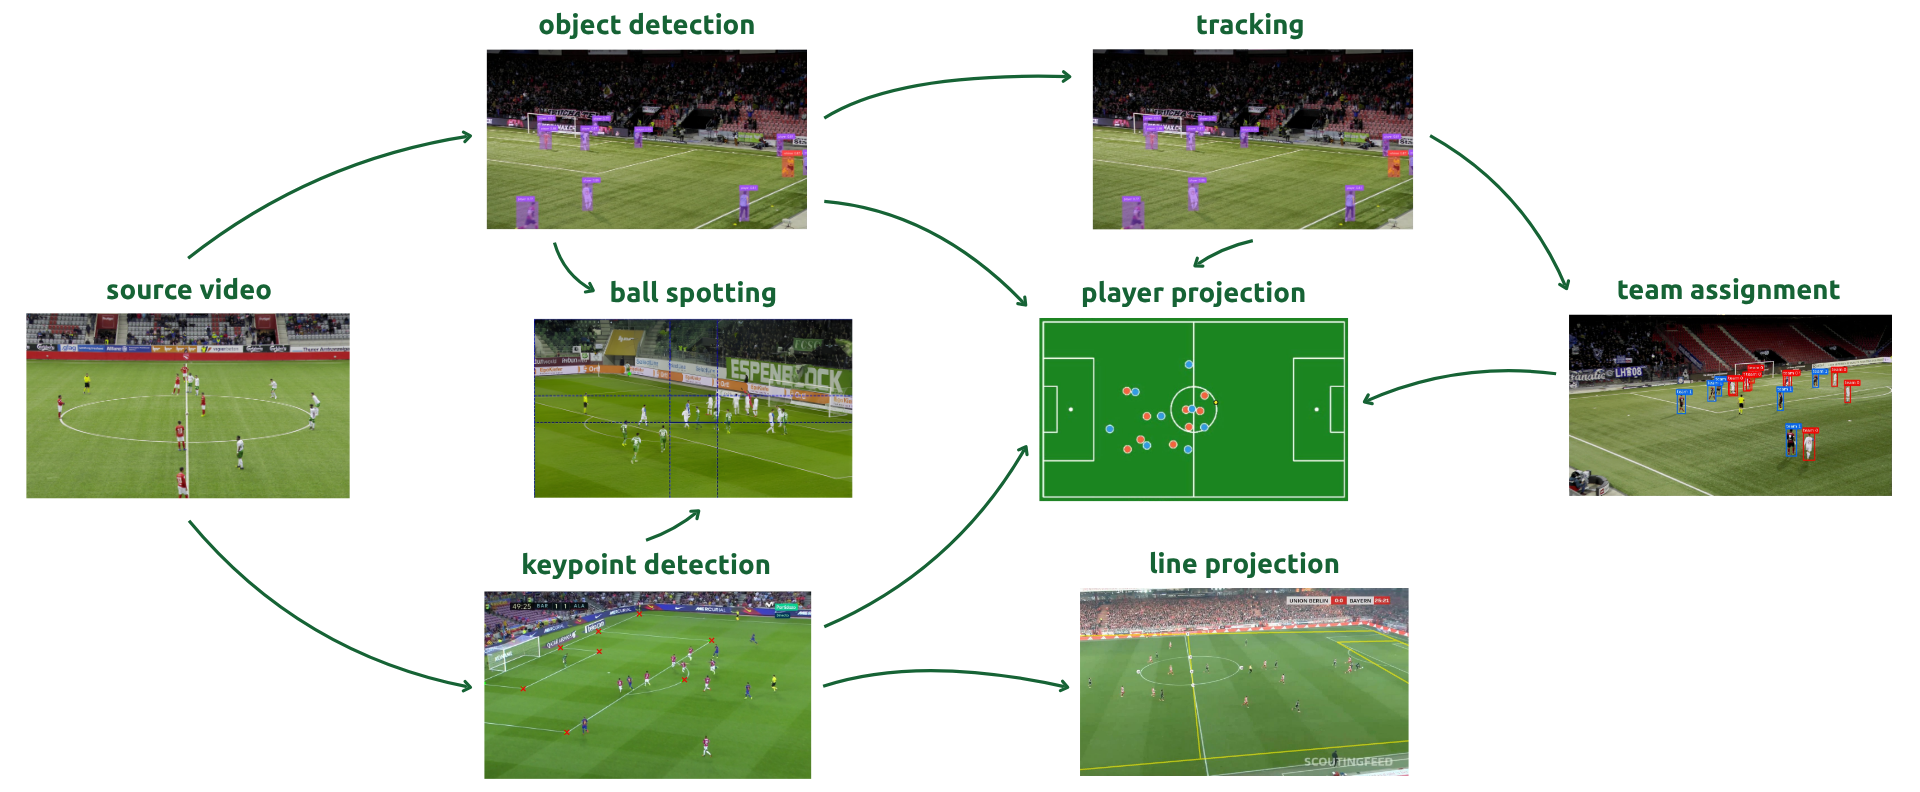
\includegraphics[width=0.95\linewidth]{figures/pipeline.png}
    \caption{Task flow diagram.}
    \label{fig:pipeline}
\end{figure}

\begin{multicols}{2}
\subsection{Object detection}
Players, referees and the ball are detected with models from the \emph{YOLO} family \cite{yolov8}, trained on the \emph{SoccerNet Tracking} dataset. For every frame of the video, the detector produces \emph{bounding boxes} for the visible objects, together with a confidence score and the corresponding class. The predictions are processed with \emph{non-maximum suppression} and then unified into a common format that feeds the tracking and team analysis stages.

\subsubsection{Player and referee detection}

For players and referees, a \emph{YOLOv11-m} base model was trained directly on the \emph{SoccerNet Tracking} data. All three available classes (players, referee and ball) were included as \textit{labels} in this training run. Because of the small size of the ball in the image and the large variability in its appearance (deformation and fast motion), however, the base model failed to detect it consistently.

In the final pipeline, therefore, the predictions of the base model are used only for the player and referee classes, in order to start the \emph{tracking} stage and the later segmentation by team.

\subsubsection{Ball detection}

A second, specialised model was trained from the weights of the base model (\emph{fine-tuning}). A new dataset was built on top of the one used for the base model, keeping the ball as the only \textit{label}.

\begin{figure}[H]
    \centering
    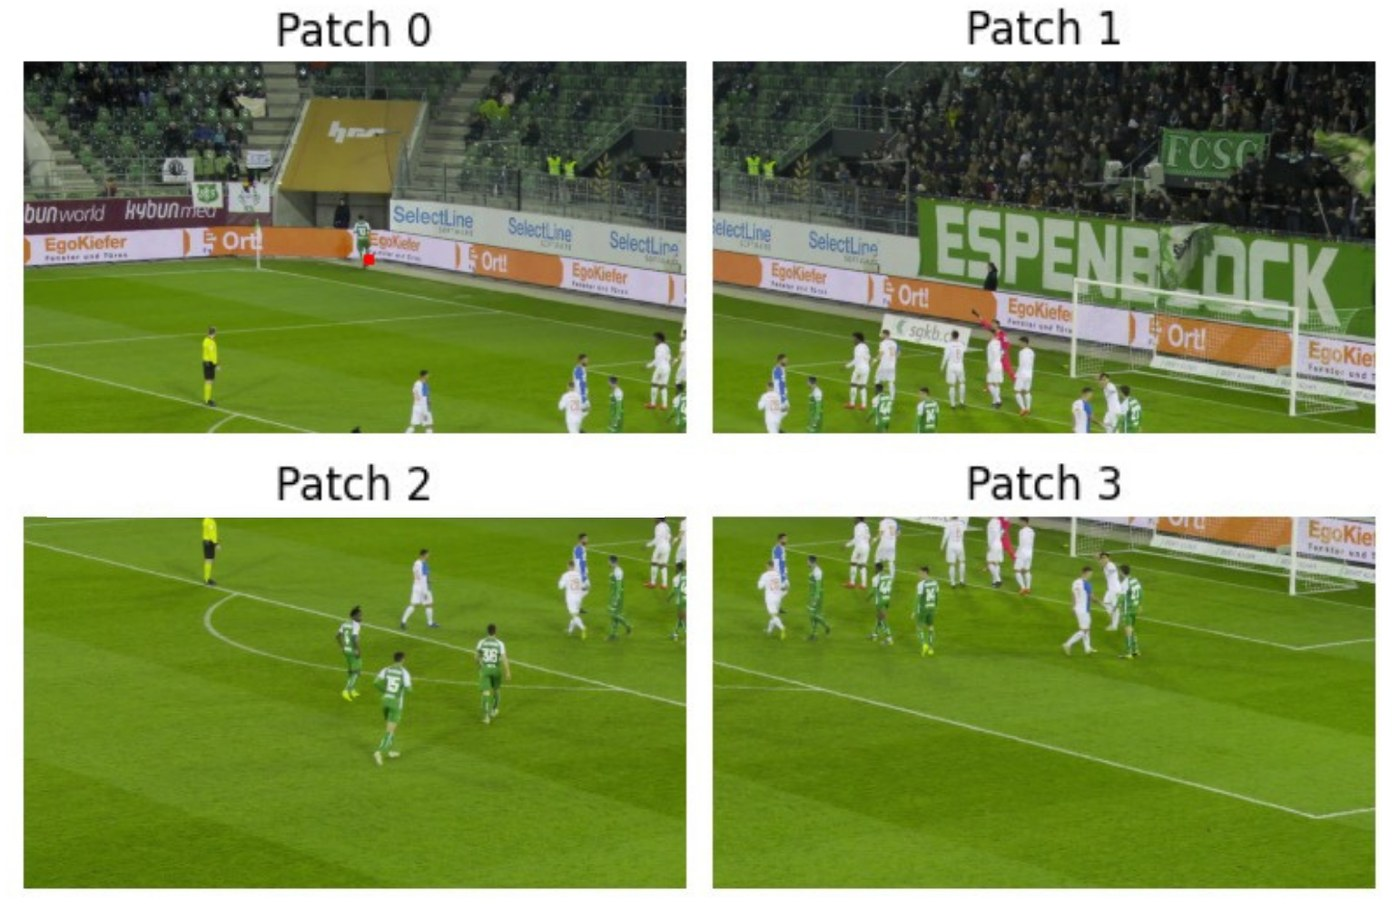
\includegraphics[width=0.96\linewidth]{figures/ball-patches.jpg}
    \caption{Splitting a frame into patches.}
    \label{fig:ball_patches}
\end{figure}

In order to improve the ball-size to image-size ratio, every frame was split into \(2 \times 2\) patches with partial overlap between them (see Figure~\ref{fig:ball_patches}), producing new images in which the ball appears larger.

The same idea is used at inference time: the full frame is processed through a \emph{slicing} scheme of overlapping patches, and the specialised ball model is applied to each of them. The detections produced in each patch are rescaled back to the original coordinate system and merged with \emph{non-maximum suppression}.

\subsection{Tracking with ByteTrack}
Frame-to-frame tracking was addressed with \emph{ByteTrack} \cite{bytetrack}, an object association method that uses both high-confidence and low-confidence detections to keep identities persistent in complex sequences. Starting from the boxes provided by the object detection model, the similarity between consecutive detections is computed using intersection over union (IoU). The resulting correspondences make it possible to reconstruct the trajectory of every player and referee over time.

\subsection{Player segmentation}

The goal of this stage is to assign each player to one of the two teams based on their kit, using only the visual information in the crops produced by YOLO and the tracker.

\begin{figure}[H]
    \centering
    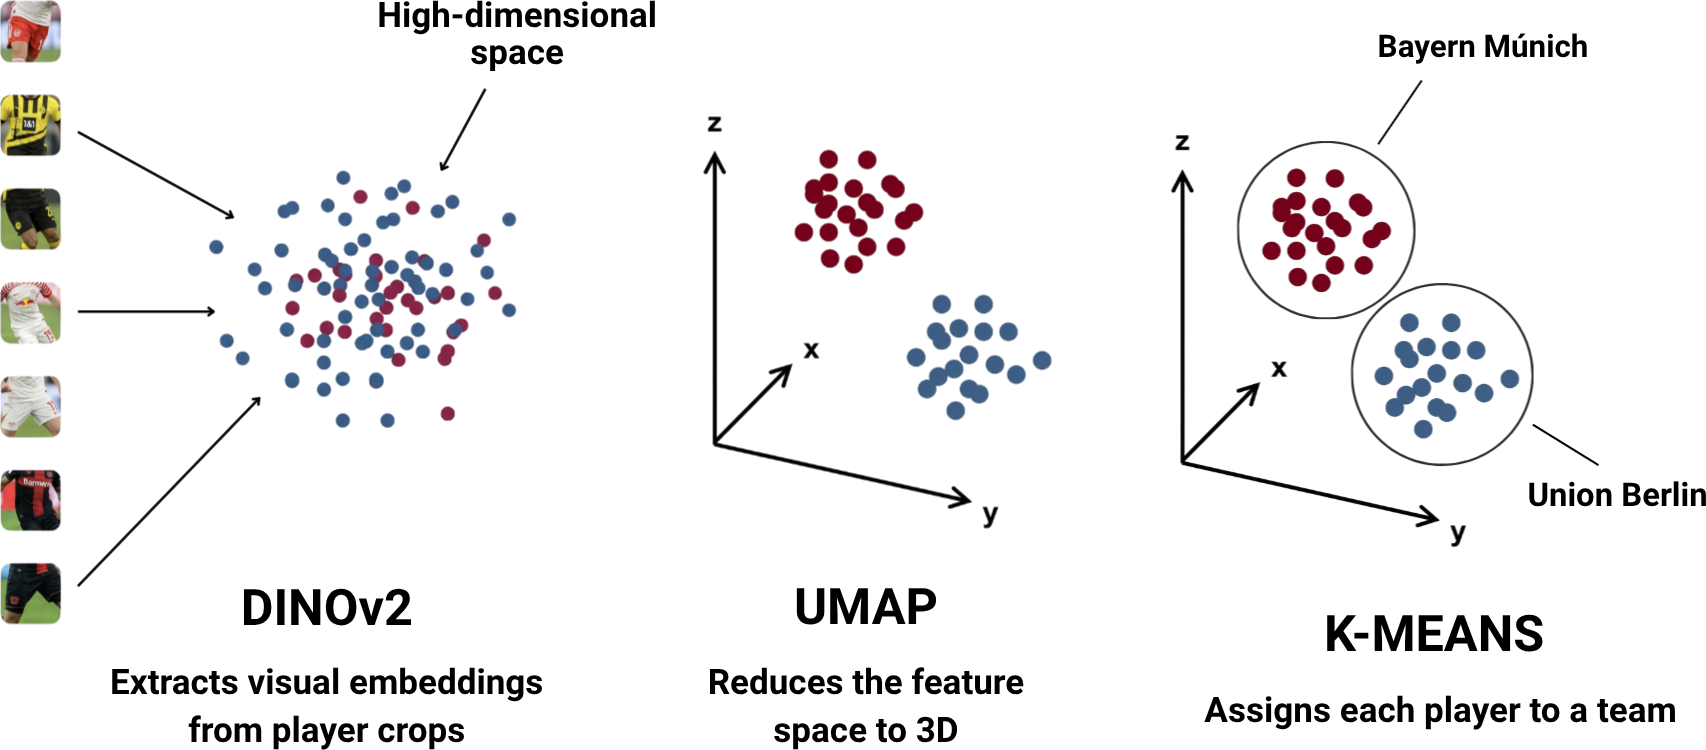
\includegraphics[width=0.96\linewidth]{figures/team-clustering.png}
    \caption{Overview of player segmentation: DINOv2 extracts appearance \emph{embeddings}, UMAP reduces the dimensionality and K-Means groups them into two teams.}
    \label{fig:segmentation_overview}
\end{figure}

\subsubsection{Appearance extraction with DINOv2}

To tell the players of each team apart, an \textit{embedding} model, \emph{DINOv2} \cite{dino}, was used. A crop centred on the \emph{bounding box} is extracted from every player detection and passed through the model, yielding a high-dimensional feature vector that captures colour and texture patterns of the clothing. These \emph{embeddings} are collected over the whole clip, associated with the tracking identifier (\emph{track id}) of each player.

\subsubsection{Dimensionality reduction with UMAP}

The vectors produced by DINOv2 live in a high-dimensional space, so \emph{UMAP} \cite{umap}, a non-linear dimensionality reduction method, was applied. At this stage the representations in $\mathbb{R}^{768}$ are projected into a reduced space $\mathbb{R}^{3}$ through a transformation that preserves the local structure of the data, which makes grouping them easier.

\subsubsection{Team grouping with K-Means and per-\emph{track} averaging}

Teams are identified automatically with the \emph{K-Means} algorithm \cite{lloyd1982least}. Rather than clustering every crop individually, the average \emph{embedding} across all of its crops over the video is computed first for each \emph{track id}. This yields a single representative vector per player, to which UMAP and then K-Means with \(K=2\) are applied. The result is a map from \emph{track id} to team, which is later used to colour every detection of that player consistently.

This scheme has two main advantages. Inference is more stable, since the team label does not change from frame to frame for the same \emph{track}; and the computational cost of the grouping drops, because it works with one point per player instead of all the individual crops.

\begin{figure}[H]
    \centering
    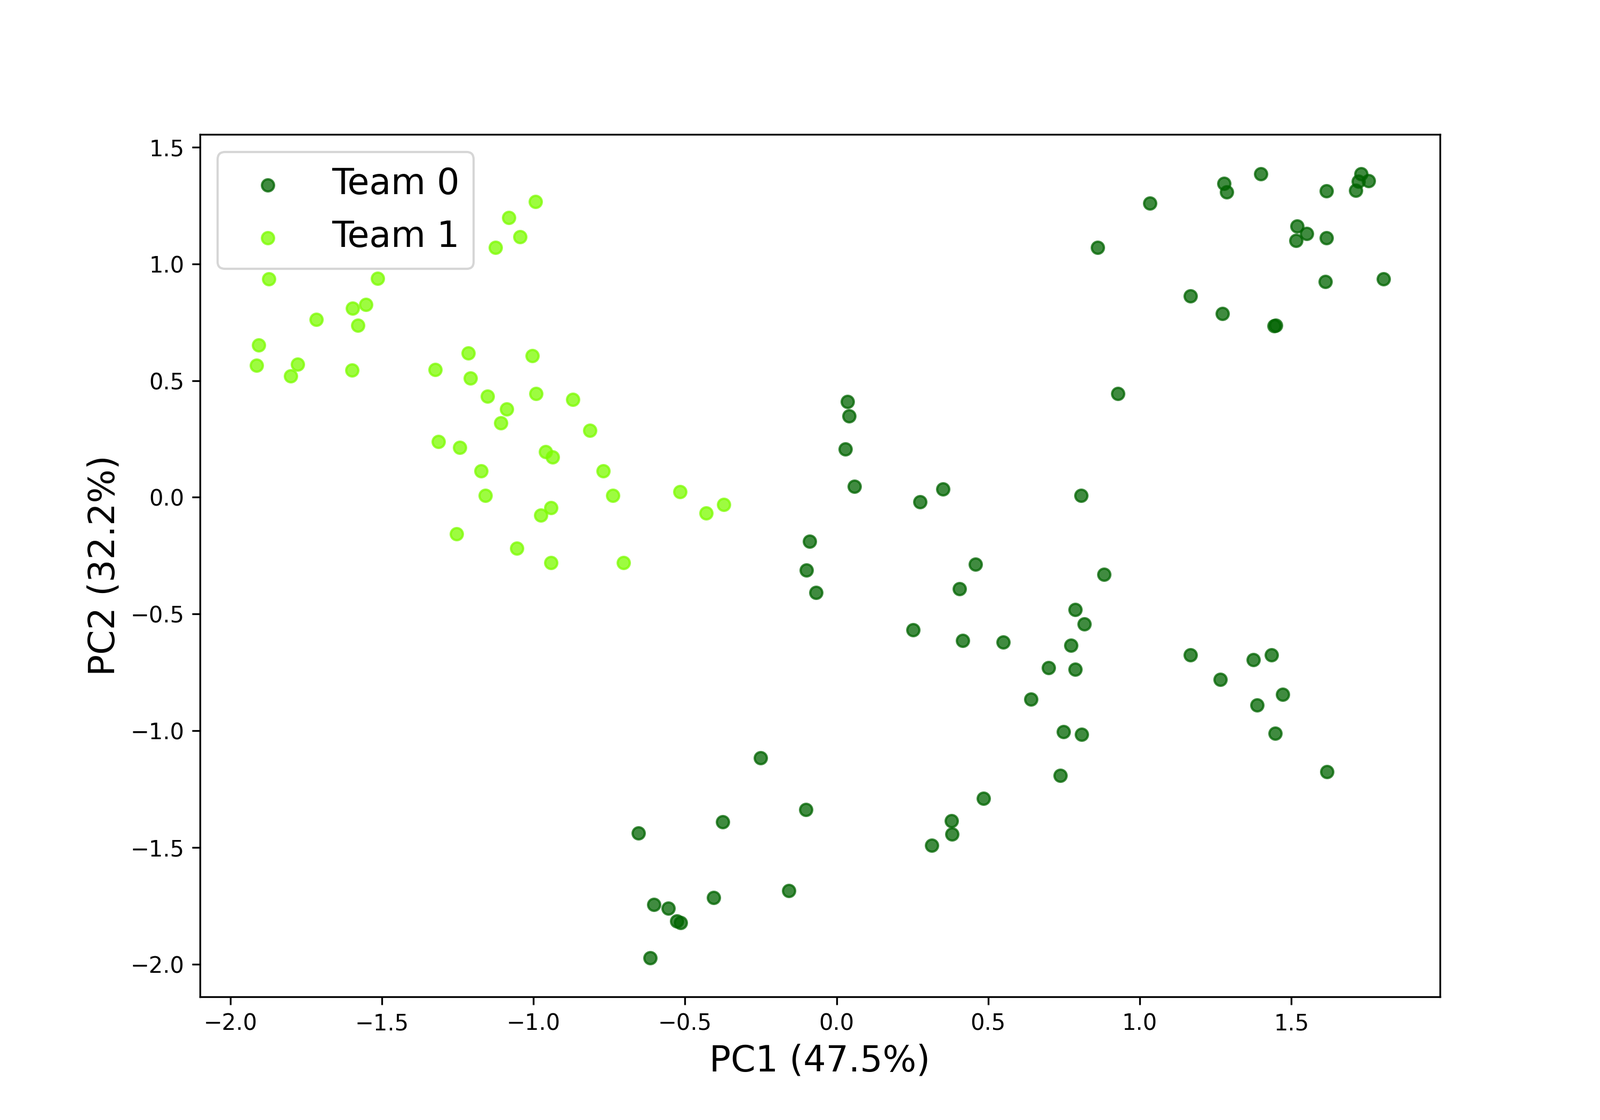
\includegraphics[width=0.96\linewidth]{figures/team-embeddings-pca.png}
    \caption{2D visualisation of the \emph{embeddings} projected with PCA. One point per \emph{track}, corresponding to the average \emph{embedding} of each player.}
    \label{fig:segmentation_pca}
\end{figure}

The teams contain more than 11 points, which is the expected maximum given that there are no more than 11 players per team. This happens because players "disappear" from the video and, when they come back into the scene, are assigned a new \textit{tracker id}.

\subsection{Keypoint detection with YOLOv8n-pose}
Reconstructing the geometry of the pitch requires a consistent set of keypoints. As explained earlier, these keypoints are not provided by SoccerNet directly: intersections, tangent points and geometric centres had to be computed to obtain the ground truth. Labels were then generated from those points in the \emph{YOLOv8n pose} format, which made it possible to train the models.

Two main configurations were defined on top of the lightweight \emph{YOLOv8n-pose} (Nano) architecture: one trained to detect the 29-keypoint dataset and another one for the 57-keypoint dataset.

A third variant was also trained using the \emph{YOLOv8x-pose} (Extra Large) architecture. The aim of this run was to assess the impact of using a model with greater capacity and computational cost compared to the lightweight versions. Only the 29-keypoint dataset was used for this comparison, in order to analyse whether the increase in network depth produced a gain in accuracy.

\subsection{Homography estimation}
With the keypoints detected in the image and their counterparts on the regulation model of the field (105\,m $\times$ 68\,m), a projective transformation was estimated using the OpenCV homography method \cite{opencv}. The homography makes it possible to map any point of the image onto the 2D plane of the playing field. To mitigate detection errors, the estimation is performed with RANSAC, which provides robustness against outliers and badly localised keypoints.

\subsection{Projection}
Finally, the estimated homography is applied to the detections and trajectories of players, referees and the ball, moving them onto the plane of the pitch. Every frame is thereby translated into a set of absolute coordinates reflecting the position of each entity on the field. This two-dimensional map shows the projected positions in real time, which makes it easier to analyse formations, movements and relevant events of the match.

\end{multicols}
